\documentclass[8pt]{article}
\usepackage[a4paper, total={16cm, 24cm}]{geometry}
\usepackage{enumitem}
\usepackage{tikz}
\usepackage{array}
\usepackage{caption}
\usepackage{anyfontsize}
\usepackage{float}

\usetikzlibrary{positioning}

\title{Appunti AESO 2025/2026}
\author{Gabriele Fiorani}
\date{\today}

\begin{document}

\maketitle

\section{\LARGE Livello dell'architettura}

Il \textbf{Livello architetturale (Instruction Set Architecture - ISA)} definisce come il processore appare ai programmatori e ai compilatori.

\begin{itemize}[left=1em, itemsep=0.5em]
    \item Non descrive \textbf{come} è costituito il processore (quello è il ruolo della microarchitettura).
    \item Si occupa invece di \textbf{cosa} il processore può fare e come il software può interagire con esso.
\end{itemize}

\noindent In pratica, è un \textbf{contratto tra hardware e software:} stabilisce le istruzioni disponibili, i registri e le modalità di accesso alla memoria.

\subsection{\Large Instruction Set Architecture - ISA}

\vspace{0.2cm}
\textbf{L'ISA (Instruction Set Architecture)} è l'insieme di tutte le \textbf{istruzioni, tipi, registri, modi di indirizzamento} e  \textbf{modalità operative} che un processore supporta. In pratica è ciò che il compilatore deve conoscere per generare codice eseguibile.

\vspace{0.5cm}  
\noindent \textbf{Componenti principali:}

\begin{itemize}[left=1em, itemsep=0.5em]
    \item \textbf{Set di istruzioni:} add, sub, load, branch...
    \item \textbf{Formato delle istruzioni:} struttura binaria, opcode, operandi
    \item \textbf{Dimensioni registri:} dimensione dei dati (registri) su cui l'architettura lavora (32 bit, 64 bit)
    \item \textbf{Tipi di dati supportati:} interi, floating point, vettori
    \item \textbf{Registri visibili al programmatore:} r0, r1, ...
    \item \textbf{Modi di indirizzamento:} diretto, indiretto, indicizzato, immediato
\end{itemize}

\noindent La lunghezza dell’istruzione dipende quindi dal design del ISA e non dalla dimensione dei registri.

\subsection{\Large Ciclo di esecuzione della CPU}

\vspace{0.2cm}

\begin{minipage}{0.45\textwidth}  % figura a sinistra
    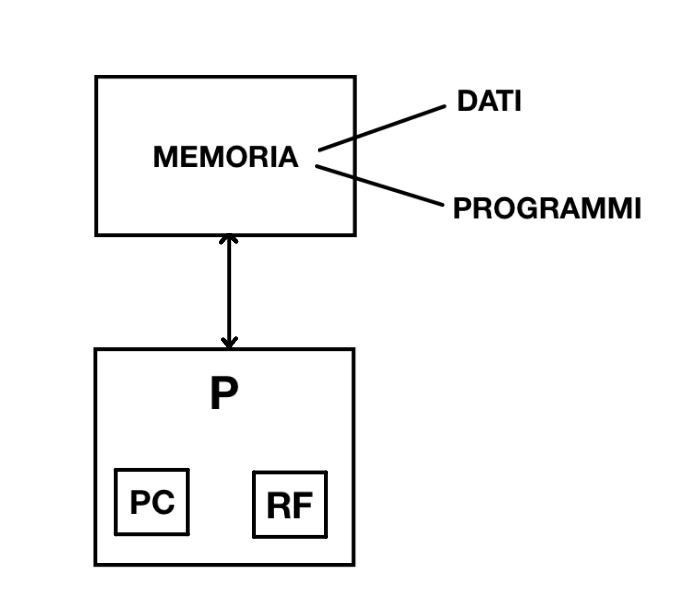
\includegraphics[width=\linewidth]{images/prima.jpg}
\end{minipage}
\hfill
\begin{minipage}{0.45\textwidth}  % codice a destra
\large
\begin{verbatim}
P == {
    while true do:
        Fetch(PC);
        Decode(Istruzione);
        Execute(Istruzione);
        Memory(Istruzione);
        WriteBack(Istruzione);
        PC = PC + 4;
}
\end{verbatim}
\end{minipage}

\vspace{0.5cm}
\begin{itemize}[left=1em, itemsep=0.5em]
    \item \textbf{Fetch:}  carica l'istruzione corrente dalla memoria all'indirizzo specificato nel  \textbf{Program Counter (PC)}. 
    \item \textbf{Decode:}  identifica il tipo di istruzione (ad esempio somma, load, store). 
    \item \textbf{Execute:} esegue l'operazione richiesta dall'istruzione. 
    \item \textbf{Memory:}  interagisce con la memoria se l'istruzione lo richiede (ad esempio in caso di load o 
store).
    \item \textbf{Write Back:}  scrive i risultati nel banco dei registri. 
    \item \textbf{Incremento PC:} Il PC viene incrementato di 4 byte per puntare alla successiva istruzione, in ARMv7 ogni istruzione è 32 bit ma la cella di memoria è 1 byte, quindi ne salta 4.
\end{itemize}

\subsection{\Large Architettura RISC e CISC}

\vspace{0.2cm}
Entrambe le architetture  sono potenti allo stesso modo, ovvero hanno la stessa espressività.

\vspace{0.5cm}
\begin{itemize}[left=1em, itemsep=0.5em]
    \item \textbf{SISC (Reduced Instruction Set Computer:} utilizza istruzioni semplici ed eseguite in un singolo ciclo di clock, favorendo la pipeline. Hanno un circuito semplice e veloce sia per la decodifica che per l’esecuzione.
    \item \textbf{CISC (Complex Instruction Set Computer):}  offre istruzioni più complesse che possono richiedere più cicli di clock, riducendo la necessità di combinare più istruzioni semplici. 
\end{itemize}

\subsection{\Large Linguaggio Macchina}

\vspace{0.2cm}
Il linguaggio macchina è il lunguaggio nativo del processore, cioè quello che la CPU è in grado di eseguire direttamente.
È costituito da sequenze di bit (0 e 1) che rappresentano operazioni specifiche e sono progettate per essere comprese dalla CPU senza necessità di traduzioni aggiuntive. Ogni tipo di CPU (o architettura) ha il proprio set di istruzioni di linguaggio macchina; quindi, il codice in linguaggio macchina è generalmente non portabile tra diverse architetture.

\subsubsection{{\fontsize{12pt}{12pt}\selectfont Caratteristiche principali:}}

\vspace{0.2cm}
\begin{itemize}[left=1em, itemsep=0.5em]
    \item \textbf{Binario:} ogni istruzione è rappresentata da combinazioni di 0 e 1.
    \item \textbf{Dipendente dall’architettura:} il linguaggio macchina è diverso per ogni tipo di CPU (x86, ARM, MIPS, ecc.).
    \item \textbf{Direttamente eseguibile:} la CPU legge le istruzioni dalla memoria e le esegue senza bisogno di traduzione.
    \item \textbf{Struttura di un’istruzione:} ogni istruzione è composta da:
	\begin{itemize}[left=1em, itemsep=0.3em]
   		 \item \textbf{Opcode:} indica l’operazione da eseguire (es. add, sub, load, store)
    		\item \textbf{Operandi:} specificano i dati su cui operare o dove salvarli (registri o indirizzi di memoria)
	\end{itemize}
    \item \textbf{Efficienza e Velocità:}  Il linguaggio macchina è il più efficiente in termini di esecuzione, poiché non richiede alcuna conversione aggiuntiva per essere eseguito dalla CPU. Si possono inoltre utilizzare i registri in modo esplicito; i registri infatti sono il sistema di memorizzazione più veloce di tutto il sistema per cui c’è uno scambio continuo tra memoria e registri.
\end{itemize}

\subsection{\Large Architettura ARMv7:}

L'ARMv7 è un'architettura RISC, progettata per massimizzare l'efficienza energetica e la velocità di esecuzione delle istruzioni. 
La CPU ARMv7 utilizza un set di \textbf{16 registri architetturali}, denominati da \textbf{R0} a \textbf{R15} , ognuno a 32 bit.

\vspace{0.5cm}
\begin{table}[h!]
\centering
\caption{Registri principali dell’architettura ARMv7}
\setlength{\tabcolsep}{10pt}
\renewcommand{\arraystretch}{1.3}
\begin{tabular}{|c|c|p{7cm}|}
\hline
\textbf{Registro} & \textbf{Nome} & \textbf{Descrizione} \\ \hline
\textbf{R0 – R12} & Generali & Registri generici per operazioni aritmetiche e logiche. \\ \hline
\textbf{R13} & SP (Stack Pointer) & Punta alla cima dello stack. \\ \hline
\textbf{R14} & LR (Link Register) & Contiene l’indirizzo di ritorno da una funzione. \\ \hline
\textbf{R15} & PC (Program Counter) & Contiene l’indirizzo dell’istruzione corrente. \\ \hline
\end{tabular}
\end{table}

\vspace{0.5cm}
\noindent Un’istruzione è composta da \textbf{Operatore}, \textbf{Destinazione}, \textbf{Sorgente1} e \textbf{Sorgente2}. 
La \textbf{Destinazione} e la \textbf{Sorgente1} sono indirizzi di registri: la loro dimensione è di 4 bit, 
sufficiente ad indirizzare i 16 (o 24) registri disponibili. 
La \textbf{Sorgente2} può essere sia un riferimento a un registro sia un \textbf{immediato}, ovvero una costante.

\subsection{\Large Linguaggio Assembly:}

\vspace{0.2cm}
Il linguaggio assembly è la forma leggibile dall'uomo del linguaggio nativo del calcolatore (linguaggio macchina).
Il linguaggio assembly, seppur di basso livello, utilizza simboli (mnemonici) per rappresentare le istruzioni, risultando più leggibile. 

\subsubsection{{\fontsize{12pt}{12pt}\selectfont Caratteristiche principali:}}
\vspace{0.2cm}
\begin{itemize}[left=1em, itemsep=0.5em]
    \item Ogni \textbf{istruzione} assembly rappresenta un’operazione elementare: somma, salto, caricamento di un valore in un registro, ecc.
    \item Utilizza \textbf{mnemonici}, cioè abbreviazioni leggibili per gli esseri umani, come MOV (move), ADD (addizione), SUB (sottrazione), CMP (confronto), B
(branch).
    \item Lavora direttamente con i registri del processore (es. R0, R1, PC, SP, ecc.).
    \item Ogni architettura (come ARM, x86, MIPS, RISC-V) ha il proprio set di istruzioni, quindi il codice Assembly non è portabile.
\end{itemize}

\begin{table}[h!]
\centering
\caption{Istruzioni aritmetiche principali dell’architettura ARMv7}
\setlength{\tabcolsep}{10pt}
\renewcommand{\arraystretch}{1.3}
\begin{tabular}{|c|p{6cm}|p{5cm}|}
\hline
\textbf{Operazione} & \textbf{Descrizione} & \textbf{Esempio} \\ \hline

\textbf{ADD} &
Somma tra due registri e salva il risultato nel registro di destinazione. &
\texttt{ADD R0, R1, R2} — R0 = R1 + R2 \\ \hline

\textbf{SUB} &
Sottrae il contenuto di due registri e memorizza nel registro di destinazione. &
\texttt{SUB R0, R1, R2} — R0 = R1 - R2 \\ \hline

\textbf{MUL} &
Moltiplica i valori di due registri e memorizza nel registro di destinazione. &
\texttt{MUL R0, R1, R2} — R0 = R1 × R2 \\ \hline

\textbf{DIV} &
Divide il contenuto di un registro per un altro (divisione intera). &
\texttt{UDIV R0, R1, R2} — R0 = R1 ÷ R2 \\ \hline

\end{tabular}
\end{table}


\begin{table}[h!]
\centering
\caption{Istruzioni logiche e di shift dell’architettura ARMv7}
\setlength{\tabcolsep}{10pt}
\renewcommand{\arraystretch}{1.3}
\begin{tabular}{|c|p{6cm}|p{5cm}|}
\hline
\textbf{Operazione} & \textbf{Descrizione} & \textbf{Esempio} \\ \hline

\textbf{AND} &
Esegue un’operazione logica AND bit a bit tra due registri e salva il risultato nel registro di destinazione. &
\texttt{AND R0, R1, R2} — R0 = R1 \&\& R2 \\ \hline

\textbf{ORR} &
Esegue un’operazione logica OR bit a bit tra due registri e salva il risultato nel registro di destinazione. &
\texttt{ORR R0, R1, R2} — R0 = R1 \(||\) R2 \\ \hline

\textbf{LSL} &
Esegue uno \textbf{shift logico a sinistra} dei bit nel registro sorgente di un numero specificato di posizioni. &
\texttt{LSL R0, R1, \#2} — R0 = \verb|R1 << 2| \\ \hline

\textbf{LSR} &
Esegue uno \textbf{shift logico a destra} riempiendo con zeri. &
\texttt{LSR R0, R1, \#2} — R0 =  \verb|R1 >> 2| (senza segno) \\ \hline

\textbf{ASR} &
Esegue uno \textbf{shift aritmetico a destra}, mantenendo il segno del numero. &
\texttt{ASR R0, R1, \#2} — R0 = \verb|R1 >> 2| (con segno) \\ \hline

\textbf{ROR} &
Esegue una \textbf{rotazione a destra} dei bit del registro sorgente. &
\texttt{ROR R0, R1, \#4} — rotazione di 4 bit a destra \\ \hline

\end{tabular}
\end{table}

\subsubsection{{\fontsize{12pt}{12pt}\selectfont Registri di uso speciale}}

Nell’architettura \textbf{ARMv7}, oltre ai registri generali (\textbf{R0–R12}), esistono tre \textbf{registri di uso speciale} fondamentali:

\begin{itemize}[left=1em, itemsep=0.5em]
    \item \textbf{PC (Program Counter) = R15}\\
    Contiene l’indirizzo dell’istruzione corrente o della prossima da eseguire. Durante il ciclo di esecuzione, il PC viene aggiornato automaticamente (ad esempio, incrementato di 4 byte dopo ogni istruzione). In pratica, indica \textit{dove si trova} il processore nel programma.

    \item \textbf{LR (Link Register) = R14}\\
    Memorizza l’indirizzo di ritorno da una funzione o subroutine. Quando si effettua una chiamata di funzione (\texttt{BL} in ARM), l’indirizzo dell’istruzione successiva viene salvato in LR, così che al termine della funzione la CPU possa ritornare al punto corretto.

    \item \textbf{SP (Stack Pointer) = R13}\\
    Punta alla cima dello \textbf{stack}, una sezione di memoria utilizzata per memorizzare variabili locali, indirizzi di ritorno e registri temporanei. Lo stack cresce verso indirizzi di memoria più bassi (\textit{dal basso verso l’alto} nel diagramma).
\end{itemize}

\vspace{0.3cm}
\noindent
La memoria del processo è organizzata in più sezioni:
\begin{itemize}[left=1em, itemsep=0.3em]
    \item \textbf{Text:} contiene il codice eseguibile del programma.
    \item \textbf{Data:} area che memorizza variabili globali e statiche.
    \item \textbf{Heap:} cresce verso indirizzi di memoria più alti, utilizzato per l’allocazione dinamica.
    \item \textbf{Stack:} cresce verso indirizzi di memoria più bassi, utilizzato per gestire chiamate di funzione e variabili locali.
\end{itemize}

\begin{center}
    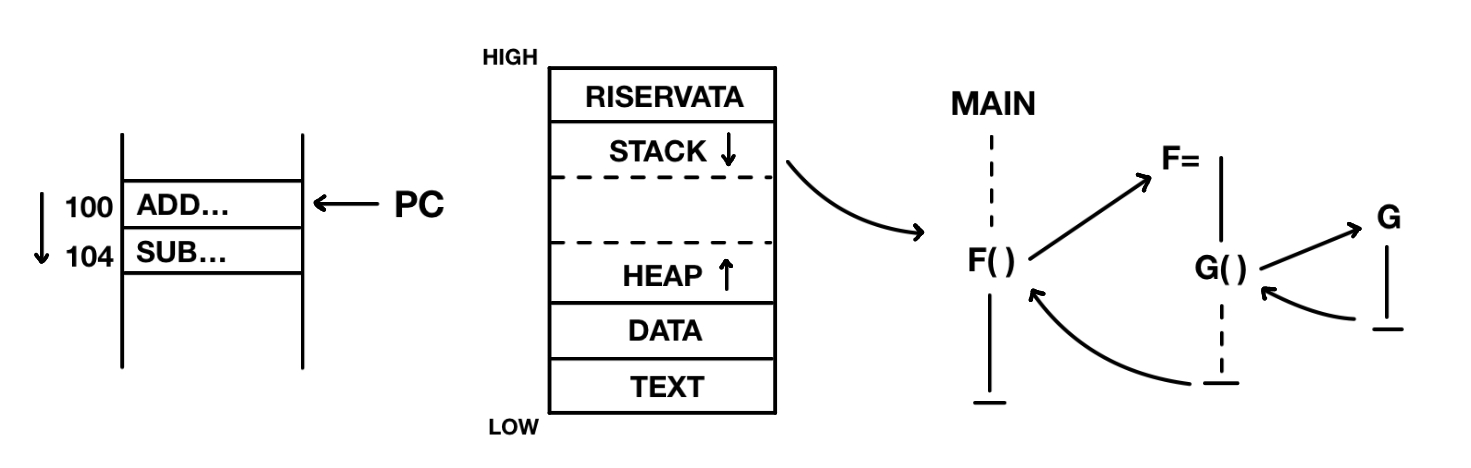
\includegraphics[width=0.9\textwidth]{images/secondo.jpg}

\end{center}

\vspace{0.3cm}
\subsubsection{{\fontsize{12pt}{12pt}\selectfont Salto condizionato e incondizionato}}
Un \textbf{salto} (in inglese jump o \textbf{branch}) è un’istruzione che modifica il normale flusso di esecuzione di un programma. Normalmente, un processore esegue le istruzioni una dopo l'altra, in ordine di memoria.
Il salto, invece, cambia questo ordine:
\begin{itemize}[left=1em, itemsep=0.3em]
    \item Dice al processore di \textbf{andare a eseguire un’altra istruzione} situata in un indirizzo diverso del programma.
    \item Questo nuovo indirizzo può essere più \textbf{avanti} (salto in avanti) o più \textbf{indietro} (salto all’indietro, usato nei cicli).
    \item Esistono due tipologie di salti:
    \begin{itemize}[left=1em, itemsep=0.3em]
        \item \textbf{Salto incondizionato:} viene sempre eseguito, indipendentemente da qualsiasi condizione. Il processore aggiorna direttamente il \textit{Program Counter} con il nuovo indirizzo di destinazione.
        \item \textbf{Salto condizionato:} viene eseguito solo se una determinata \textit{condizione logica} è vera (ad esempio, se un registro vale zero o se un confronto restituisce “uguale”). In caso contrario, l’esecuzione prosegue normalmente.
    \end{itemize}
\end{itemize}

\vspace{0.3cm}
\subsubsection{{\fontsize{12pt}{12pt}\selectfont L'istruzione "Compare"}}
In Assembly, l’istruzione \textbf{CMP} (abbreviazione di compare, “confronta”) serve per \textbf{confrontare due valori}, ma \textbf{non memorizza il risultato}: modifica solo i {flag} nel registro dei flag, in base alla differenza tra gli operandi.

\begin{table}[H]
\centering
\caption{Principali \textbf{flag} modificati da \textbf{CMP}}
\setlength{\tabcolsep}{10pt}
\renewcommand{\arraystretch}{1.3}
\begin{tabular}{|c|p{4cm}|p{7cm}|}
\hline
\textbf{Flag} & \textbf{Significato} & \textbf{Quando è impostato (1)} \\ \hline

\textbf{ZF} (Zero Flag) &
Il risultato è zero. &
\texttt{A == B}  \\ \hline

\textbf{SF} (Sign Flag) &
Il risultato è negativo. &
\texttt Il bit più significativo del risultato è 1 \\ \hline

\textbf{CF} (Carry Flag) &
C'è stato un "prestito". &
\texttt{A} $<$ \texttt{B} (per numeri senza segno) \\ \hline

\textbf{OF} (Overflow Flag) &
Overflow aritmetico. &
\texttt La differenza non entra nel range (\textbf{con segno}) \\ \hline

\end{tabular}
\end{table}

\newpage
\noindent \textbf{Esercizio - calcolo del fattoriale:}


\vspace{0.3cm}
\begin{center}
\noindent
\begin{minipage}{0.6\linewidth}
\begin{verbatim}
    .text
    .global fact
    .type fact, %function

fact:
    MOV R1, R0       @ Copia il parametro in R1
    MOV R0, #1       @ Inizializza il risultato a 1

start:
    CMP R1, #0       @ Confronta R1 con 0
    BEQ fine         @ Se uguale, vai a fine
    MUL R0, R0, R1   @ R0 = R0 * R1
    SUB R1, R1, #1   @ Decrementa R1
    B start          @ Ripeti il ciclo

fine:
    MOV PC, LR       @ Ritorna al chiamante
\end{verbatim}
\end{minipage}
\end{center}


\end{document}
